\section{多目标优化}

\begin{definition}[帕累托前沿]
    Pareto Front 没有完美的唯一解，但我们可以找到最优的权衡解，这些最优权衡解的集合称为帕累托前沿。
\end{definition}

\begin{definition}[帕累托最优解]
    一个无法在不牺牲任何其他目标的情况下，单独提升某一个目标的解。在帕累托前沿上的任何一辆车，如果你想让它的性能变得更好，那么它的油耗或成本就必然会变差。
\end{definition}

\subsection{NSGA-II 算法}

\begin{definition}[NSGA-II 算法]
    \texttt{NSGA-II} 是一种高效的多目标遗传算法。它的执行过程像是在模拟“优胜劣汰”的自然选择。
\end{definition}

\begin{tips}
    NSGA-II 算法采用精英策略，父代个体与子代个体合并后进行快速非支配排序，并且用拥挤度的概念代替了共享半径，扩大了产生下一代个体时的筛选范围。
\end{tips}

算法流程图如下所示：

\begin{figure}[H]
    \centering
    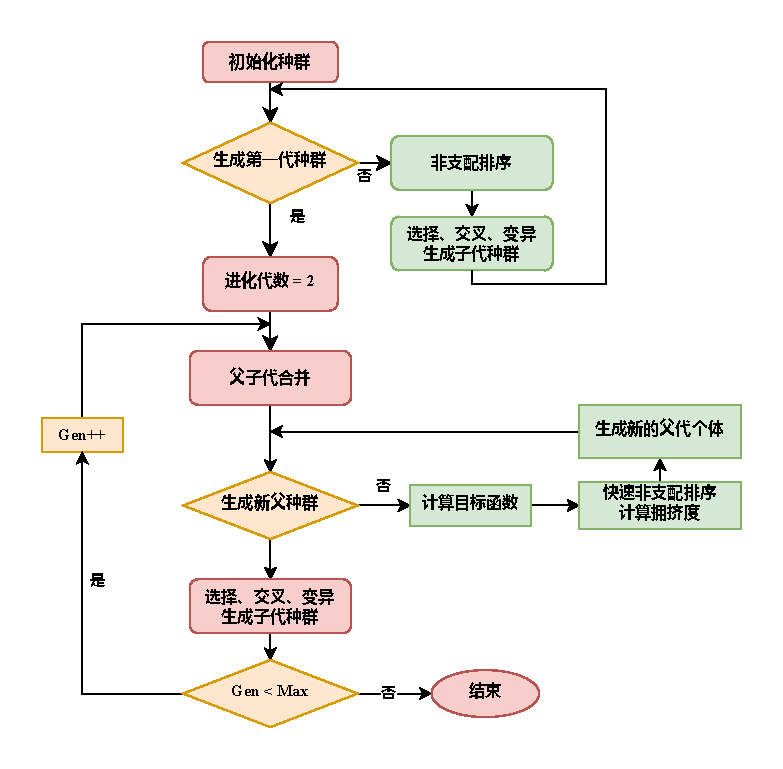
\includegraphics[width=0.8\textwidth]{chapters/多目标优化/images/多目标优化/NSGA-II.drawio.pdf}
    \caption{NSGA-II 算法流程图}
    \label{fig:nsga-ii-flowchart}
\end{figure}

其中，交叉操作模拟自然界中染色体交叉换位的现象，用于生成新个体，决定了算法的全局搜索能力。标准的 NSGA-II 算法使用二进制模拟交叉算子，第 $k+1$ 代个体的计算公式为：
$$
    \begin{aligned}
         & p_{1, \lambda+1}=\frac{1}{2}\left[\left(1-\beta_{q j}\right) p_{1, \lambda}+\left(1+\beta_{q j}\right) p_{2, \lambda}\right] \\
         & p_{2, \lambda+1}=\frac{1}{2}\left[\left(1+\beta_{q j}\right) p_{1, k}+\left(1-\beta_{q j}\right) p_{2, \lambda}\right]
    \end{aligned}
$$

